\documentclass[aspectratio=1610]{beamer}
\usepackage{graphicx}

\graphicspath{{./v3.5/}}
\DeclareRobustCommand\SUTname{TOPAS-nBio (TOPAS v3.5)}
\DeclareRobustCommand\benchmarkname{TOPAS-nBio (TOPAS v3.4)}


\title{\SUTname}
\subtitle{Regression testing (cf.\ \benchmarkname)}
\author{Jos\'e Ramos-M\'endez}
\institute{University of California San Francisco}
\date{\today}



\begin{document}

\frame{\titlepage}

\begin{frame}
  \frametitle{Table of contents}
  \tableofcontents
\end{frame}




\section{DBSCAN}

\begin{frame}{\secname}
 \begin{columns}
  \begin{column}{0.4\linewidth}
   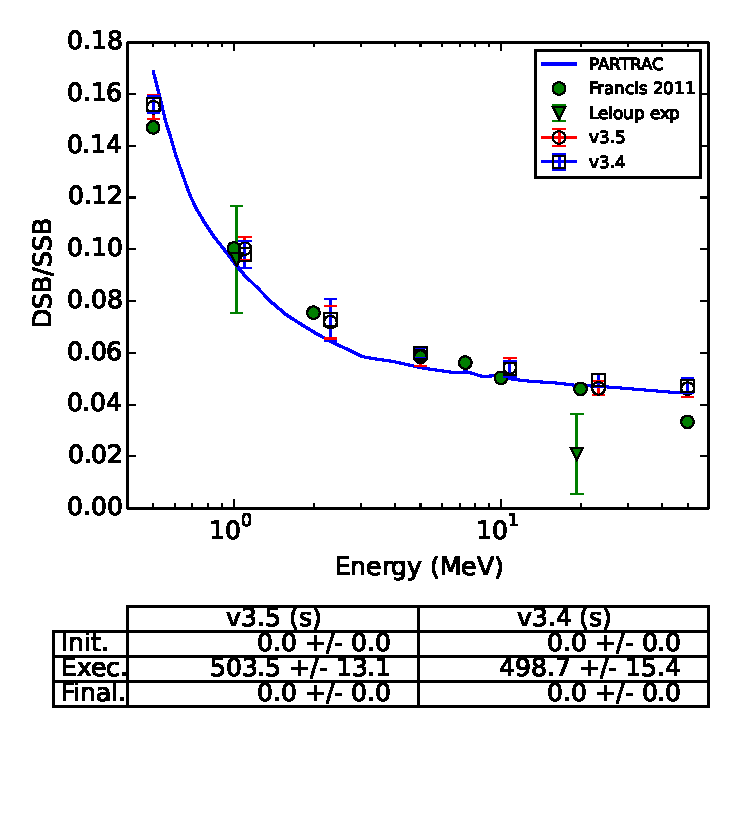
\includegraphics[width=1.1\textwidth]{DBSCAN2}
  \end{column}
  \begin{column}{0.6\linewidth} 
   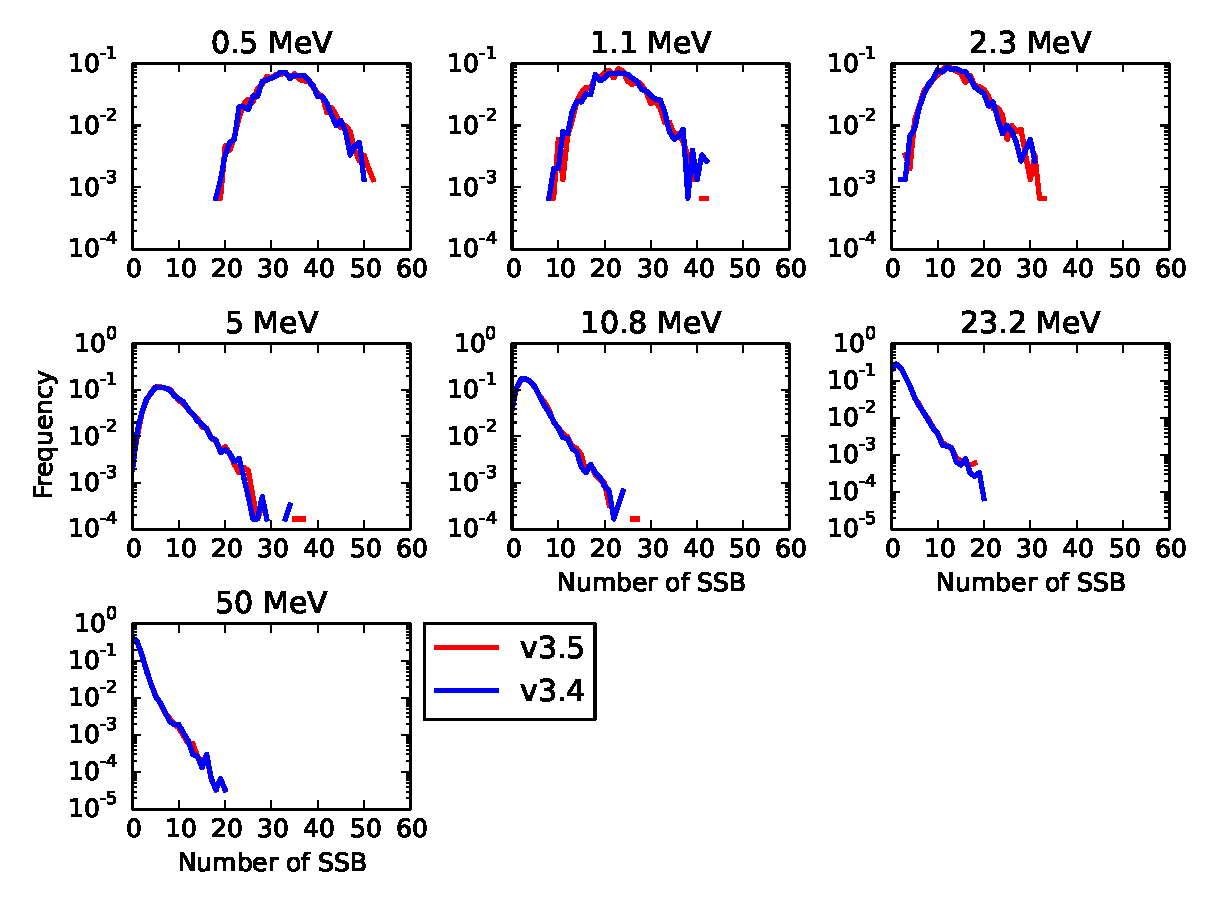
\includegraphics[width=\textwidth]{DBSCAN1}
  \end{column}
 \end{columns}
\begin{itemize}
\item \tiny{Francis Z, Villagrasa C, Clairand I. Simulation of DNA damage clustering after proton irradiation using an adapted DBSCAN algorithm. \textit{Comput Methods Programs Biomed}. 2011; 101(3):265-270. doi:10.1016/j.cmpb.2010.12.012}
\end{itemize}
\end{frame}

\section{G-value: step-by-step}

\begin{frame}{\secname}
 \centering
   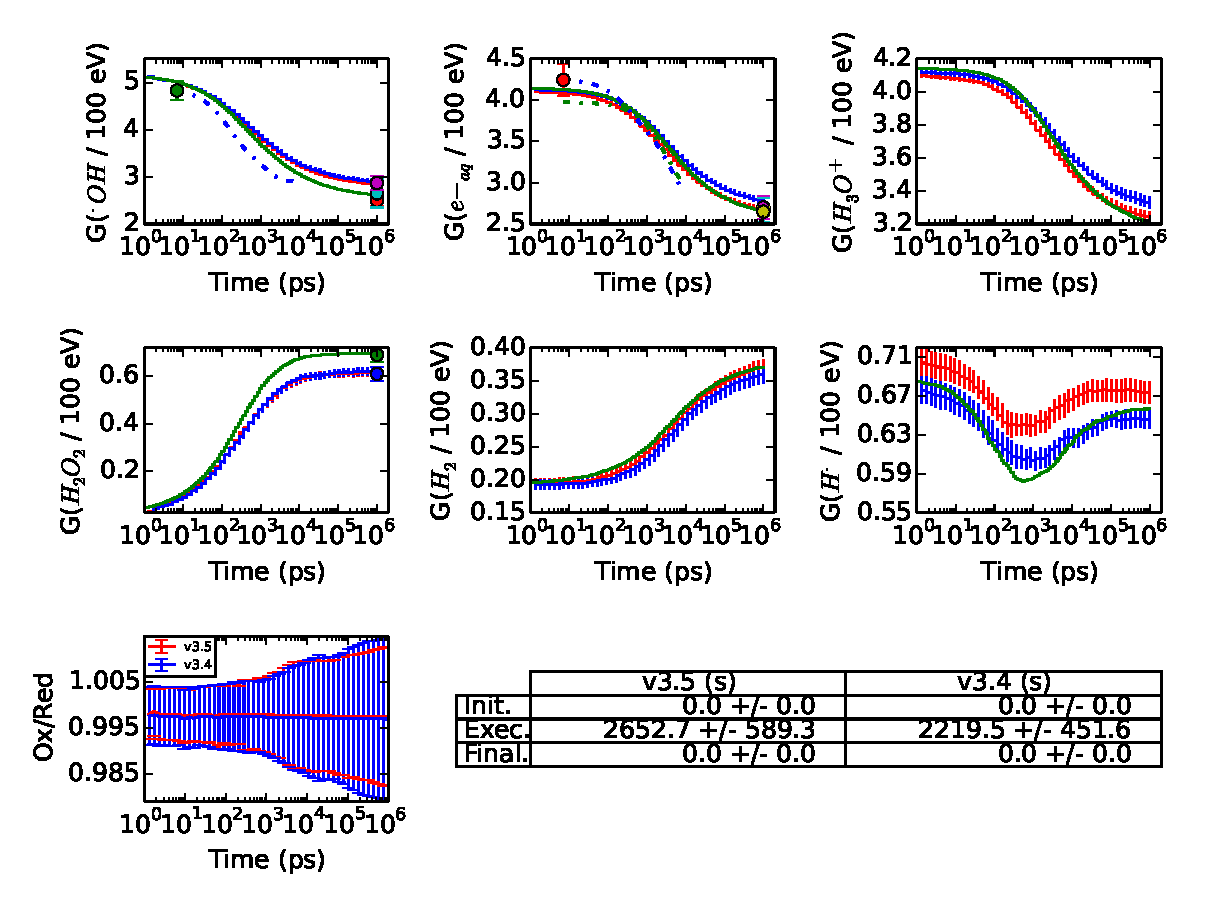
\includegraphics[width=0.75\textwidth]{Gvalue}
\begin{itemize}
\item \tiny{Wang F, Schmidhammer U, Larbre JP, Zong Z, Marignier JL, Mostafavi M. Time-dependent yield of the hydrated electron and the hydroxyl radical in D$_{2}$O: A picosecond pulse radiolysis study. Phys Chem Chem Phys. 2018;20(23):15671-15679. doi:10.1039/c8cp02276c}
\end{itemize}
\end{frame}

\section{G-value: IRT}

\begin{frame}{\secname}
 \centering
  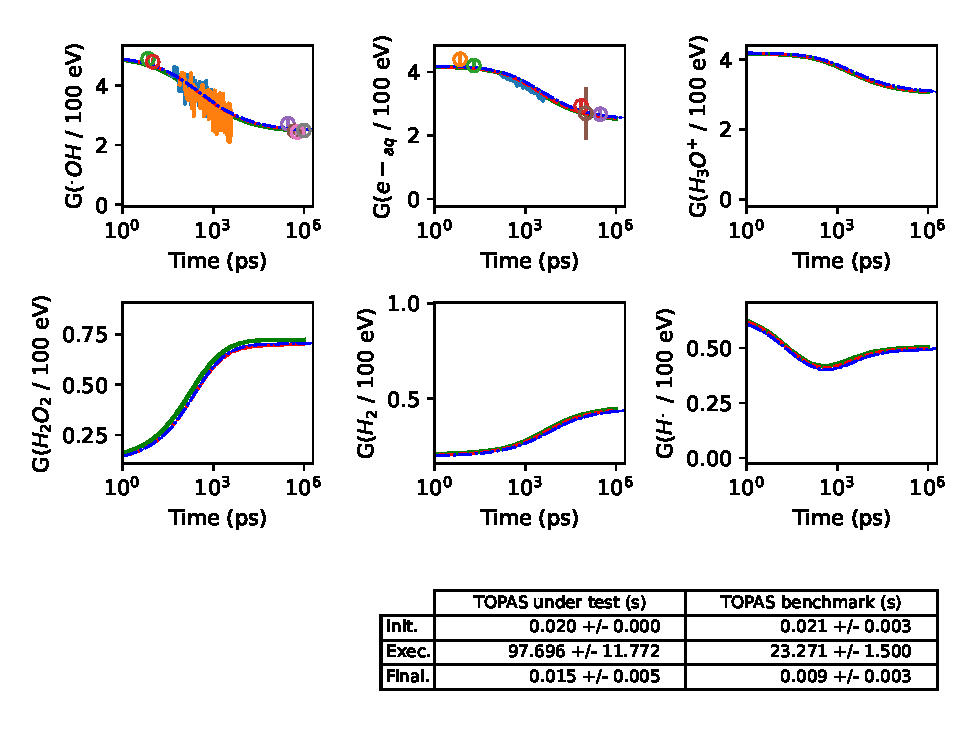
\includegraphics[width=0.75\textwidth]{GvalueIRT}
\end{frame}

\section{LET}

\begin{frame}{\secname}
 \centering
   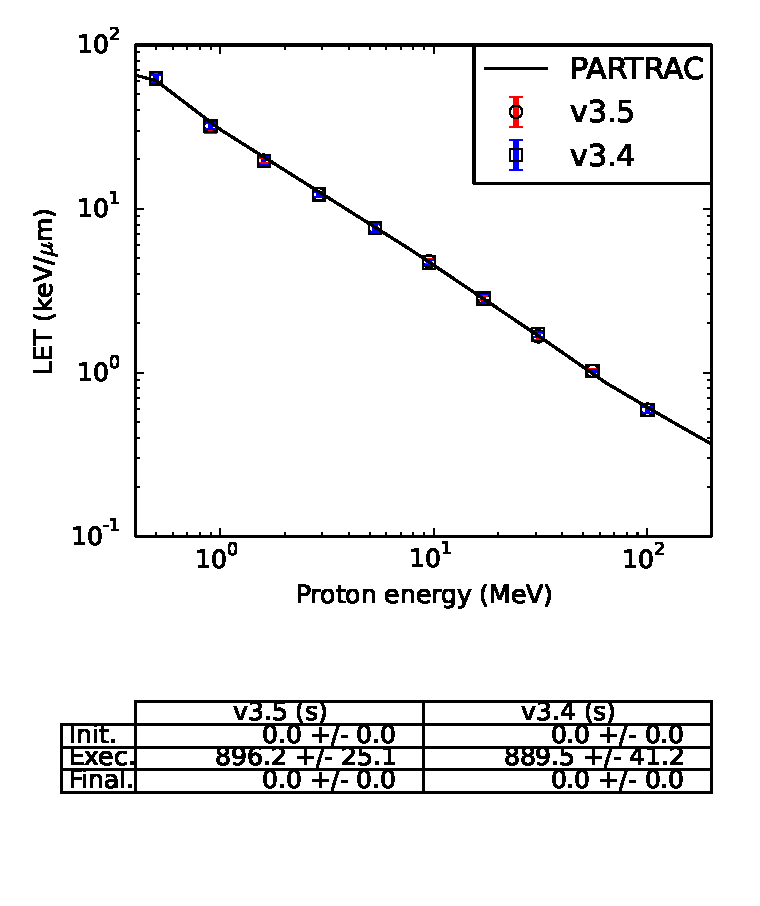
\includegraphics[width=0.5\textwidth]{LET}
\end{frame}

\section{Nanodosimetry I}

\begin{frame}{\secname}
 \centering
   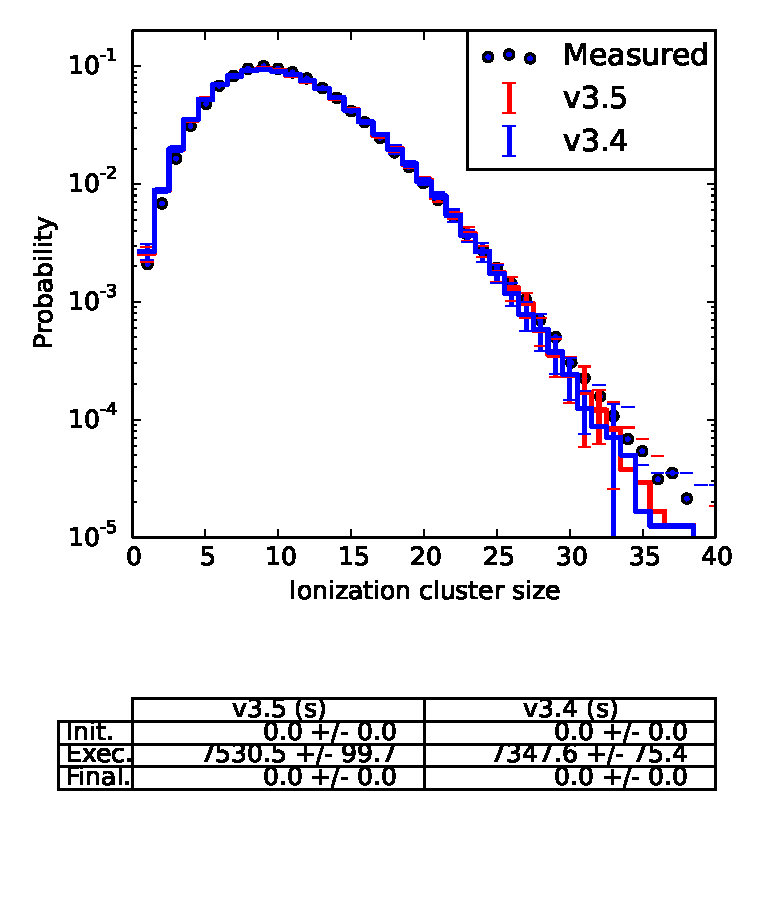
\includegraphics[width=0.5\textwidth]{NanodosimetryI}
\begin{itemize}
 \item \tiny{Conte V, Selva A, Colautti P, et al., Nanodosimetry: Towareds a new concept of radiation quality. \textit{Radiat Prot Dosimetry}. 2018;180(1-4):150-156. doi:10.1093/rpd/ncx175}
\end{itemize}
\end{frame}


\section{Nanodosimetry II}

\begin{frame}{\secname}
 \centering
   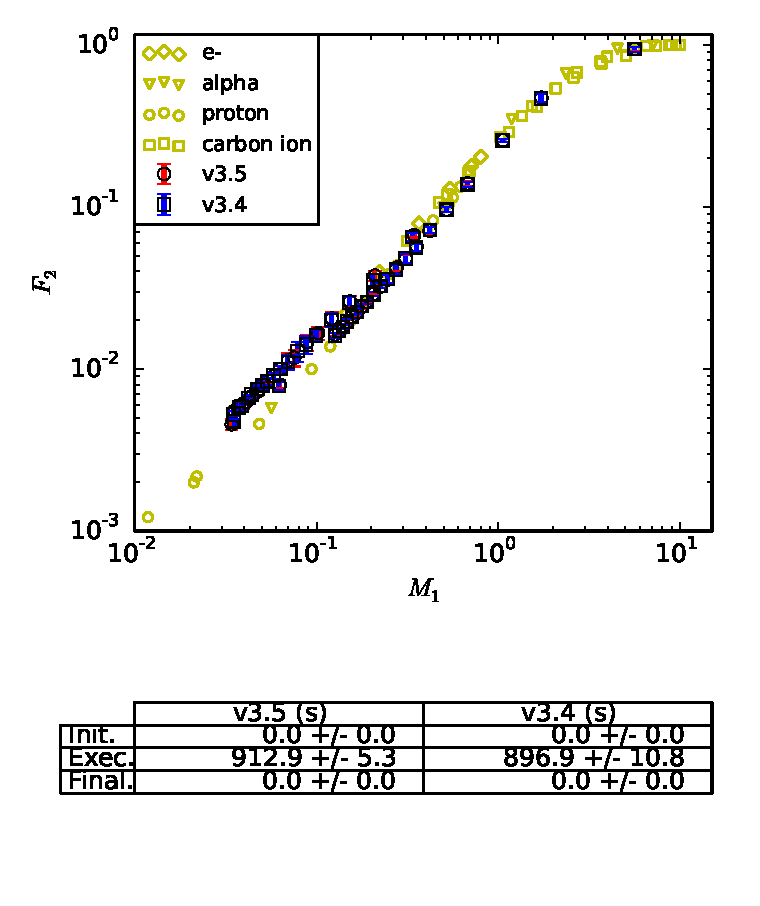
\includegraphics[width=0.5\textwidth]{NanodosimetryII}
\begin{itemize}
 \item \tiny{Conte V, Selva A, Colautti P, et al., Nanodosimetry: Towareds a new concept of radiation quality. \textit{Radiat Prot Dosimetry}. 2018;180(1-4):150-156. doi:10.1093/rpd/ncx175}
\end{itemize}
\end{frame}


\section{Nanodosimetry III}

\begin{frame}{\secname}
 \centering
   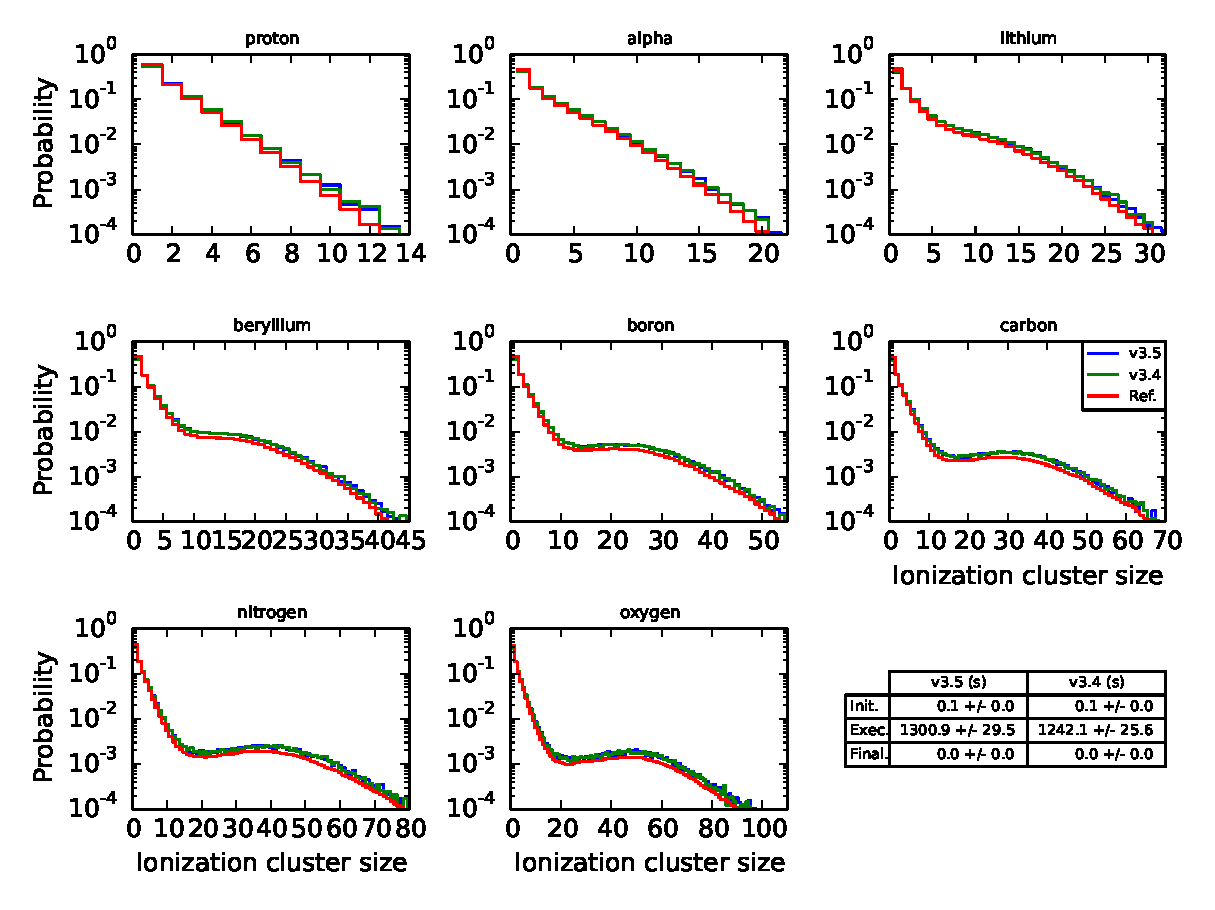
\includegraphics[width=0.75\textwidth]{NanodosimetryIII}
\begin{itemize}
 \item \tiny{Ramos-M\'endez J, Burigo LN, Schulte R, Chuang C, Faddegon B. Fast calculation of nanodosimetric quantities in treatment planning of proton and ion therapy. \textit{Phys Med Biol.} 2018;63(23):235015. doi:10.1088/1361-6560/aaeeee}
\end{itemize}
\end{frame}

\end{document}
